\clearpage
\VerdierPhysicalPageAnchor{0097}%
\begingroup
\setlength{\abovedisplayskip}{3pt plus 2pt minus 2pt}%
\setlength{\belowdisplayskip}{3pt plus 2pt minus 2pt}%
\setlength{\jot}{2pt}%
\VerdierSemanticAnchor{ch1-3-3-4}
\noindent\textbf{命題 3.3.4. (TRIII)}\quad
\begingroup\itshape
\VerdierSemanticAnchor{ch1-3-3-4-triii}
$K(C)$ の二つの完全三角

\VerdierSemanticAnchor{ch1-3-3-4-source-triangles}
\begin{equation*}
  X\xrightarrow{u}Y\xrightarrow{v}Z\xrightarrow{w}X[1],
  \qquad
  X'\xrightarrow{u'}Y'\xrightarrow{v'}Z'\xrightarrow{w'}X'[1]
\end{equation*}
と、$K(C)$ における可換正方形

\VerdierSemanticAnchor{ch1-3-3-4-eq1}
\begin{equation}
  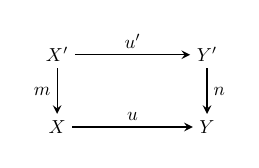
\begin{tikzpicture}[>=stealth,baseline=(current bounding box.center),scale=0.68,
    every node/.style={transform shape}]
    \node (Xp) at (0,1.35) {$X'$}; \node (Yp) at (2.8,1.35) {$Y'$};
    \node (X)  at (0,0) {$X$};   \node (Y)  at (2.8,0) {$Y$};
    \draw[->] (Xp) -- node[above] {$u'$} (Yp);
    \draw[->] (Xp) -- node[left] {$m$} (X);
    \draw[->] (Yp) -- node[right] {$n$} (Y);
    \draw[->] (X) -- node[above] {$u$} (Y);
  \end{tikzpicture}
  \tag{3.3.4.1}
\end{equation}
を考える。
\VerdierSemanticAnchor{ch1-3-3-4-filler}
図式

\VerdierSemanticAnchor{ch1-3-3-4-morphism-diagram}
\begin{center}
  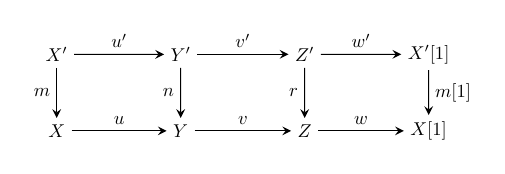
\begin{tikzpicture}[>=stealth,scale=0.67,every node/.style={transform shape}]
    \node (Xp)  at (0,1.45) {$X'$};
    \node (Yp)  at (2.35,1.45) {$Y'$};
    \node (Zp)  at (4.70,1.45) {$Z'$};
    \node (Xps) at (7.05,1.45) {$X'[1]$};
    \node (X)   at (0,0) {$X$};
    \node (Y)   at (2.35,0) {$Y$};
    \node (Z)   at (4.70,0) {$Z$};
    \node (Xs)  at (7.05,0) {$X[1]$};
    \draw[->] (Xp) -- node[above] {$u'$} (Yp);
    \draw[->] (Yp) -- node[above] {$v'$} (Zp);
    \draw[->] (Zp) -- node[above] {$w'$} (Xps);
    \draw[->] (X) -- node[above] {$u$} (Y);
    \draw[->] (Y) -- node[above] {$v$} (Z);
    \draw[->] (Z) -- node[above] {$w$} (Xs);
    \draw[->] (Xp) -- node[left] {$m$} (X);
    \draw[->] (Yp) -- node[left] {$n$} (Y);
    \draw[->] (Zp) -- node[left] {$r$} (Z);
    \draw[->] (Xps) -- node[right] {$m[1]$} (Xs);
  \end{tikzpicture}
\end{center}
\VerdierSemanticAnchor{ch1-3-3-4-morphism-conclusion}
が三角の射となるような射 $r\colon Z'\longrightarrow Z$ が存在する。
\endgroup

\VerdierSemanticAnchor{ch1-3-3-4-proof}
定義により、与えられた三角は次の形の三角に同型である：

\VerdierSemanticAnchor{ch1-3-3-4-cone-models}
\begin{align*}
  V&\xrightarrow{\dot f}W\xrightarrow{\dot p(f)}c(f)
     \xrightarrow{\dot q(f)}V[1],\\
  V'&\xrightarrow{\dot f'}W'\xrightarrow{\dot p(f')}c(f')
     \xrightarrow{\dot q(f')}V'[1],
\end{align*}
\VerdierSemanticAnchor{ch1-3-3-4-square-reduction}
したがって、正方形 (3.3.4.1) は次の正方形に同型である：

\VerdierSemanticAnchor{ch1-3-3-4-homotopy-class-square}
\begin{center}
  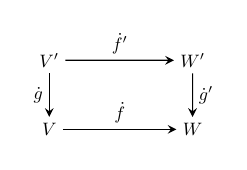
\begin{tikzpicture}[>=stealth,scale=0.65,every node/.style={transform shape}]
    \node (Vp) at (0,1.35) {$V'$}; \node (Wp) at (2.8,1.35) {$W'$};
    \node (V)  at (0,0) {$V$};   \node (W)  at (2.8,0) {$W$};
    \draw[->] (Vp) -- node[above] {$\dot f'$} (Wp);
    \draw[->] (Vp) -- node[left] {$\dot g$} (V);
    \draw[->] (Wp) -- node[right] {$\dot g'$} (W);
    \draw[->] (V) -- node[above] {$\dot f$} (W);
  \end{tikzpicture},
\end{center}
\VerdierSemanticAnchor{ch1-3-3-4-representatives}
ここで $g\colon V'\longrightarrow V$ と $g'\colon W'\longrightarrow W$ は
$\operatorname{comp}(C)$ の射である。$\operatorname{comp}(C)$ における正方形

\VerdierSemanticAnchor{ch1-3-3-4-comp-square}
\begin{center}
  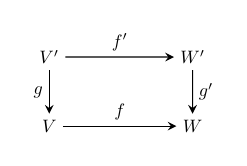
\begin{tikzpicture}[>=stealth,scale=0.65,every node/.style={transform shape}]
    \node (Vp) at (0,1.35) {$V'$}; \node (Wp) at (2.8,1.35) {$W'$};
    \node (V)  at (0,0) {$V$};   \node (W)  at (2.8,0) {$W$};
    \draw[->] (Vp) -- node[above] {$f'$} (Wp);
    \draw[->] (Vp) -- node[left] {$g$} (V);
    \draw[->] (Wp) -- node[right] {$g'$} (W);
    \draw[->] (V) -- node[above] {$f$} (W);
  \end{tikzpicture}
\end{center}
\VerdierSemanticAnchor{ch1-3-3-4-open-conclusion}
\endgroup

